\chapter{The Case\label{case}}
In this chapter an overview to the studied component is given.
Also we are going to peek into the architecture of each environment and how they are related to the component.

\section{Overview of the Component}
The studied component is written in JavaScript using Node.js.
Its response time is critical to the application.
The component can not be scaled horizontally.

\begin{figure}
    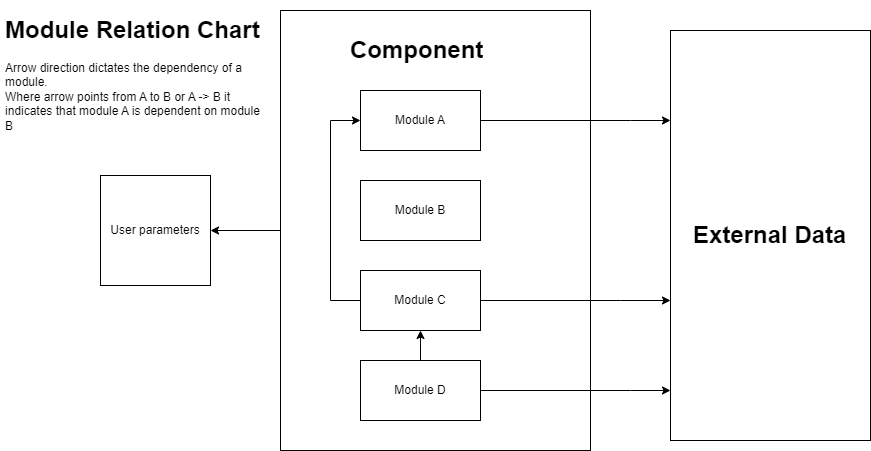
\includegraphics[width=\textwidth]{images/modules_relation_uml.png}
    \caption{Components modules and their dependencies.}
    \label{figure:module:relation}
\end{figure}
\begin{figure}
    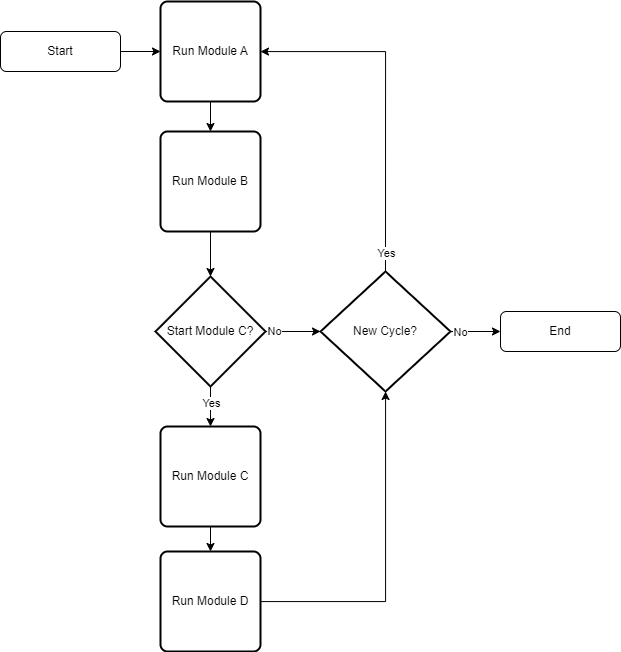
\includegraphics[width=\textwidth]{images/module_flow_chart.png}
    \caption{Modules flowchart. Modules are run inside the component.}
    \label{figure:module:flow}
\end{figure}

The component contains four modules A, B, C and D.
Some modules are dependent on external data and some are dependent on other modules.
The dependencies can be seen in figure \ref{figure:module:relation}.
%All response times for data fetching are excluded from the performance review.

Modules run in cycles where one full cycle contains successful performance from all modules A to D.
The modules are run in sequence one by one from A to D.
Any error interrupts the cycle and ends the process.

The \textbf{module A} is the first module in the sequence.
It is the first module of the cycle and is always called.

The \textbf{module B} is the second module in the sequence.
It is independent from other modules and it runs after \textbf{module A}.

The \textbf{module C} is the third module in the sequence.
It runs after \textbf{module B} only when response from \textbf{module A} requires it to run.

The \textbf{module D} is the final module in the sequence.
It is run after \textbf{module C}.
After the module performs its operations the cycle restart from the \textbf{module A}.

The sequence of the modules are shown in figure \ref{figure:module:flow}.
Note that error at any point of the sequence ends the process.

When any of the modules fails to perform its task an error is raised and the cycle is interrupted.
When modules are running without errors the modules A and B are always performed. 
The modules C and D are run only when the data from \textbf{module A} requires them to run.
Each module waits for the response of every external call before continuing their process.

\section{Monolith Overview}
The monolith uses Node.js version 14.19.1. The node version runs using V8 engine version \textit{8.4.371.23-node.85}.

The monolith application is a three tier application containing user interface, server side and database.
The server side contains four components.
One of the components is the component studied in this research.
The component is run independently from other components.
In appendix \ref{appendix:architecture:monolith} the overall architecture of the monolith application can be seen.

\section{The Independent Service}
The independent service uses Node.js version 14.18.3.
The node version uses v8 engine version \textit{8.4.371.23-node.85}.

The service contains the component studied in this research and some functionality that allows communication with the component.
The architecture of the whole application including the independent service can be seen in appendix \ref{appendix:architecture:microservices}

\section{Summary}
This research studies performance of a server side JavaScript software component.
Performance is defined as components response time excluding all calls outside the component.
Component is written using JavaScript with Node.js.
The component performance is measured in two different environments.
First environment is the one where the component is a part of monolith environment.
In the second environment the component is refactored from the monolith environment into independent service.
The component is not modified between environments.
